\documentclass[11pt,a4paper]{article}

% ── Packages ──
\usepackage[utf8]{inputenc}
\usepackage[T1]{fontenc}
\usepackage{lmodern}
\usepackage[margin=1in]{geometry}
\usepackage{amsmath,amssymb}
\usepackage{graphicx}
\usepackage{booktabs}
\usepackage{hyperref}
\usepackage{listings}
\usepackage{xcolor}
\usepackage{tikz}
\usetikzlibrary{arrows.meta, positioning, shapes.geometric}
\usepackage{algorithm}
\usepackage{algpseudocode}
\usepackage{enumitem}
\usepackage{caption}

% ── Code listing style ──
\definecolor{codebg}{RGB}{250,250,250}
\definecolor{codegreen}{RGB}{40,160,40}
\definecolor{codegray}{RGB}{128,128,128}
\definecolor{codepurple}{RGB}{150,50,180}

\lstdefinestyle{pythonstyle}{
    backgroundcolor=\color{codebg},
    basicstyle=\ttfamily\small,
    keywordstyle=\color{codepurple}\bfseries,
    commentstyle=\color{codegreen},
    stringstyle=\color{orange},
    numberstyle=\tiny\color{codegray},
    breaklines=true,
    frame=single,
    rulecolor=\color{gray!40},
    numbers=left,
    numbersep=5pt,
    tabsize=4,
    language=Python,
    showstringspaces=false,
}

\lstset{style=pythonstyle}

% ── Metadata ──
\title{\textbf{Preference Learning Pipeline for MidiBERT-Piano}:\\
       \large Dataset Generation and Reward Model Fine-Tuning for Symbolic Music}
\author{Aditya Kinjawadekar}
\date{March 2026}

\begin{document}

\maketitle

% ══════════════════════════════════════════════════════════════════════════════
\begin{abstract}
Evaluating and aligning generative models for symbolic music remains a significant challenge due to the subjective nature of musical quality and the absence of robust automatic metrics. Reinforcement Learning from Human Feedback (RLHF) offers a promising solution, but requires a pre-trained reward model capable of judging musical coherence. We present a complete, end-to-end preference learning pipeline built on top of MidiBERT-Piano~\cite{midibertpiano}. The framework consists of two primary components: (1) a sophisticated dataset generator that tokenizes MAESTRO v3.0.0 MIDI files into Compound Word (CP) representation and produces $n^{2}$ preference pairs via a suite of targeted corruption strategies (simulating structural, harmonic, and rhythmic degradation); and (2) a parameter-efficient fine-tuning (PEFT) script that attaches a scalar reward head to the MidiBERT encoder, training it with a Bradley--Terry preference loss using Low-Rank Adaptation (LoRA). This expansive document provides the necessary theoretical context, architectural motivations, and implementation details for the pipeline.
\end{abstract}

% ══════════════════════════════════════════════════════════════════════════════
\section{Introduction and Motivation}

Generative models for symbolic music, typically based on Transformer architectures, have achieved remarkable success in composing realistic piano performances. However, these models are traditionally trained via maximum likelihood estimation (MLE) on datasets of human performances. MLE training forces the model to mimic the training data distribution but fails to distinguish between high-quality compositions and mediocre ones, nor does it explicitly discourage structurally incoherent generations.

In natural language processing, Reinforcement Learning from Human Feedback (RLHF) has bridged this gap by aligning language models with human preferences. The RLHF pipeline relies on a \textbf{Reward Model (RM)} that assigns a scalar quality score to a generated sequence. To train an RM for music, we require a dataset of preference pairs: instances where one musical excerpt is explicitly preferred over another.

Collecting human preference data for music is notoriously expensive and time-consuming. To bootstrap the RM, we employ a \textbf{synthetic preference dataset} strategy. By taking high-quality, human-performed classical music (the MAESTRO dataset) and applying controlled, musically-destructive corruption algorithms, we can automatically generate pairs where the original, uncorrupted version is unconditionally preferred. 

% ══════════════════════════════════════════════════════════════════════════════
\section{Background: Symbolic Music Representation}

A fundamental decision in processing symbolic music is the choice of tokenization. Historically, formats like MIDI-like or REMI (Revamped MIDI-derived events) flatten all musical events (Note-On, Note-Off, Velocity, Time-Shift) into a 1D sequence. This flattening breaks the semantic grouping of note attributes, forcing the Transformer to learn that a ``Pitch'' token is intrinsically linked to the preceding ``Duration'' token.

\subsection{Compound Word (CP) Tokenization}

MidiBERT~\cite{midibertpiano} adopts the \textbf{Compound Word (CP)} representation~\cite{cp_representation}, drastically reducing sequence length and explicitly grouping note attributes. In CP, a single token is not a single integer, but a \textbf{4-tuple} representing four distinct characteristics of a note event.

Let $\mathbf{t}$ be a CP token. It is defined as:
\begin{equation}
    \mathbf{t} = \bigl[\,t_{\text{Bar}},\; t_{\text{Pos}},\; t_{\text{Pitch}},\; t_{\text{Dur}}\,\bigr]
\end{equation}

\begin{itemize}
    \item \textbf{Bar ($t_{\text{Bar}}$)}: Indicates whether this token begins a new bar (\texttt{Bar New}) or continues an existing one (\texttt{Bar Continue}). Vocabulary size: 4 (includes padding and masking).
    \item \textbf{Position ($t_{\text{Pos}}$)}: Represents the onset time of the note within the current bar, discretized into 16 bins. Vocabulary: 18 (16 fractions + pad + mask).
    \item \textbf{Pitch ($t_{\text{Pitch}}$)}: The MIDI pitch value, typically restricted to the 88 piano keys (MIDI notes 22 to 109). Vocabulary: 90 (88 pitches + pad + mask).
    \item \textbf{Duration ($t_{\text{Dur}}$)}: The length of the note, quantized into 64 distinct time bins ranging from 60 ticks to 3840 ticks. Vocabulary: 66 (64 bins + pad + mask).
\end{itemize}

\subsection{MidiBERT Embedding Strategy}

Because the token is multi-dimensional, MidiBERT embeds each of the four attributes independently into a $d_{\text{attr}} = 256$ dimensional space using separate learned lookup tables. These four embeddings are then concatenated to form a 1024-dimensional vector, which is linearly projected down to the BERT hidden size ($d_{\text{model}} = 768$).

\begin{equation}
    \mathbf{h}_{\text{emb}} = W_{\text{proj}}\,\bigl[\,
        E_{\text{Bar}}(t_{\text{Bar}})\;\|\;
        E_{\text{Pos}}(t_{\text{Pos}})\;\|\;
        E_{\text{Pitch}}(t_{\text{Pitch}})\;\|\;
        E_{\text{Dur}}(t_{\text{Dur}})
    \,\bigr]
\end{equation}

This architecture allows the attention mechanism to directly access and correlate independent musical features simultaneously, rather than waiting for recurrent updates across a 1D sequence.

% ══════════════════════════════════════════════════════════════════════════════
\section{Dataset Generation Pipeline}
\label{sec:dataset}

The first script in our pipeline, \texttt{generate\_preference\_dataset.py}, processes the MAESTRO v3.0.0 dataset~\cite{maestro}. MAESTRO contains ~200 hours of virtuosic piano performances. 

\subsection{Standardizing and Tokenizing}

We utilize the preprocessing tools native to the MidiBERT repository to ensure exact compatibility with the pre-trained weights.
\begin{enumerate}
    \item \textbf{Parsing}: The \texttt{miditoolkit} library extracts Note and Tempo objects.
    \item \textbf{Quantization}: Musical time is Continuous. We quantize it to a discrete grid with a resolution of 480 ticks per quarter note. Note onsets are snapped to the nearest 120-tick boundary.
    \item \textbf{Grouping and Conversion}: Notes are grouped chronologically by Bar. The tuples are mapped to integer IDs using the pre-computed \texttt{CP.pkl} dictionary (or extracted from the checkpoint state dict).
    \item \textbf{Chunking}: Since BERT models have quadratic attention complexity, sequence length is bounded. We slice the CP sequences into non-overlapping chunks of $L = 512$ tokens. Sequences shorter than 512 are padded with a designated 4-tuple \texttt{[Bar<PAD>, Pos<PAD>, Pitch<PAD>, Dur<PAD>]}.
\end{enumerate}

\subsection{Targeted Corruption Strategies}

To construct preference pairs, we must simulate the types of objective errors a generative model might make. We implemented five corruption strategies that operate directly on the discrete CP token dimension arrays.

\begin{table}[h]
\centering
\caption{Detailed definitions of the CP token corruption strategies used to generate negative preference examples.}
\label{tab:corruption}
\begin{tabular}{@{}p{3.5cm}p{11.5cm}@{}}
\toprule
\textbf{Strategy} & \textbf{Musical Motivation \& Implementation} \\
\midrule
\texttt{shuffle\_bars} & \textbf{Tests structural coherence}. Generative models often produce locally coherent music that wanders globally. We identify bar boundaries (where $t_{\text{Bar}}$ = \texttt{Bar New}), split the sequence into bar-level blocks, and randomly shuffle these blocks. This destroys macroscopic structure while preserving local within-bar harmony. \\
\addlinespace
\texttt{randomize\_pitch} & \textbf{Tests harmonic mapping}. We replace the $t_{\text{Pitch}}$ integer for every non-padding token with a random sample from a uniform distribution $\mathcal{U}(0, 87)$. The rhythm remains pristine, but the resultant audio sounds highly dissonant. \\
\addlinespace
\texttt{randomize\_position} & \textbf{Tests rhythmic jitter}. Models sometimes struggle with micro-timing. We replace the $t_{\text{Pos}}$ integer (the sub-bar fraction) with uniform noise. Notes occur at the correct bar, and play the correct pitch for the correct duration, but their onsets are chaotic. \\
\addlinespace
\texttt{note\_dropout} & \textbf{Tests sparsity and continuity}. We randomly drop 40\% of the tokens. To restore the tensor to length 512, we append padding tokens at the end. This simulates a model ``forgetting'' to play notes, leaving awkward silences. \\
\addlinespace
\texttt{randomize\_duration} & \textbf{Tests articulation loss}. We replace $t_{\text{Dur}}$ with uniform noise. This alters the musical phrasing (staccato vs legato) without changing the melody or rhythm. \\
\bottomrule
\end{tabular}
\end{table}

\subsection{Generating $\mathcal{O}(n^2)$ Pairs}

If we tokenize $n$ unique MIDI segments, producing $n$ original token arrays and $n$ corrupted variants, we generate the full Cartesian product to maximize dataset size and contrastive diversity:

\begin{equation}
    \mathcal{D} = \bigl\{\,(\mathbf{x}_i^{\text{orig}},\;\mathbf{x}_j^{\text{corrupt}},\;y=1) \;\big|\; i,j \in \{1,\ldots,n\}\,\bigr\}
\end{equation}

By pairing original file $i$ with the corruption of file $j$, the RM must learn that \textit{any} clean, human-composed piece is preferable to \textit{any} structurally broken piece, preventing the model from merely memorizing specific songs.

% ══════════════════════════════════════════════════════════════════════════════
\section{Reward Model Architecture and Fine-Tuning}
\label{sec:model}

The second script, \texttt{finetune\_reward\_model.py}, transforms the pre-trained, masked-language-model MidiBERT into a discriminative Reward Model.

\subsection{Architecture}

The RM processes an input sequence $\mathbf{X} \in \mathbb{Z}^{512 \times 4}$ and outputs a single scalar value $r \in \mathbb{R}$.

\begin{figure}[h]
\centering
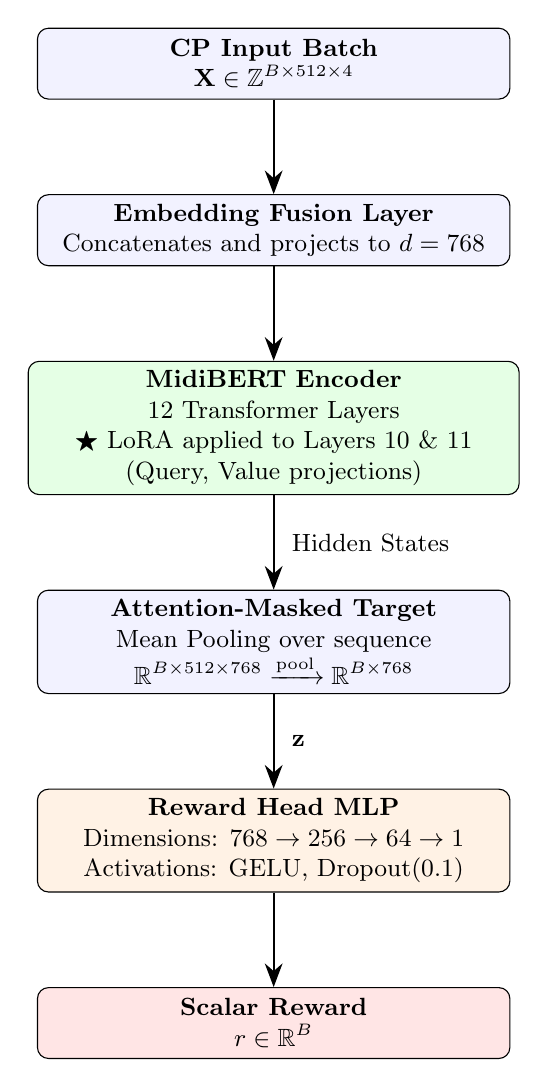
\begin{tikzpicture}[
    node distance=1.2cm,
    block/.style={rectangle, draw, rounded corners, minimum width=6cm, minimum height=0.9cm, align=center, fill=blue!5, font=\small},
    arrow/.style={-{Stealth[length=3mm]}, thick},
]
    \node[block] (input) {\textbf{CP Input Batch}\\ $\mathbf{X} \in \mathbb{Z}^{B \times 512 \times 4}$};
    \node[block, below=of input] (emb) {\textbf{Embedding Fusion Layer} \\ Concatenates and projects to $d=768$};
    \node[block, below=of emb, fill=green!10, text width=6cm] (bert) {\textbf{MidiBERT Encoder} \\ 12 Transformer Layers \\ $\bigstar$ LoRA applied to Layers 10 \& 11 \\ (Query, Value projections)};
    \node[block, below=of bert] (pool) {\textbf{Attention-Masked Target} \\ Mean Pooling over sequence \\ $\mathbb{R}^{B \times 512 \times 768} \xrightarrow{\text{pool}} \mathbb{R}^{B \times 768}$};
    \node[block, below=of pool, fill=orange!10] (head) {\textbf{Reward Head MLP} \\ Dimensions: $768 \to 256 \to 64 \to 1$ \\ Activations: GELU, Dropout($0.1$)};
    \node[block, below=of head, fill=red!10] (out) {\textbf{Scalar Reward} \\ $r \in \mathbb{R}^{B}$};

    \draw[arrow] (input) -- (emb);
    \draw[arrow] (emb) -- (bert);
    \draw[arrow] (bert) -- (pool) node[midway, right, xshift=0.1cm] {\small Hidden States};
    \draw[arrow] (pool) -- (head) node[midway, right, xshift=0.1cm] {\small $\mathbf{z}$};
    \draw[arrow] (head) -- (out);
\end{tikzpicture}
\caption{The end-to-end Reward Model architecture. The base MidiBERT model is frozen, and only the LoRA adapters (green) and the newly initialized Reward Head (orange) are updated during gradient descent.}
\label{fig:architecture}
\end{figure}

Due to CP padding, sequences vary in effective length. Simple mean pooling would incorrectly include padding tokens in the aggregate state. We use \textbf{Attention-Masked Mean Pooling}:

\begin{equation}
    \mathbf{z} = \text{LayerNorm}\!\left(\frac{\sum_{i=1}^{L} m_i \cdot \mathbf{h}_i}{\sum_{i=1}^{L} m_i}\right) \quad \text{where} \quad m_i = \begin{cases} 1 & \text{if } t_{\text{Bar}, i} \neq \text{\texttt{Bar<PAD>}} \\ 0 & \text{otherwise} \end{cases}
\end{equation}

\subsection{Parameter-Efficient Fine-Tuning (PEFT)}

Training a 85M parameter BERT model from scratch on small datasets is prone to catastrophic forgetting and overfitting. Rather than full fine-tuning, we utilize \textbf{Low-Rank Adaptation (LoRA)}~\cite{hu2022lora}.

LoRA freezes the pre-trained weights $W_0 \in \mathbb{R}^{d \times k}$ and injects trainable rank decomposition matrices into each layer:
\begin{equation}
    W_{\text{forward}} = W_0 + \Delta W = W_0 + \frac{\alpha}{r_{rank}} B A
\end{equation}
where $B \in \mathbb{R}^{d \times r_{rank}}$ and $A \in \mathbb{R}^{r_{rank} \times k}$. 

We target the self-attention \textbf{Query} and \textbf{Value} matrices of the \textbf{last 2 layers} of the 12-layer encoder (layers 10 and 11). For $r_{rank}=8$ and $\alpha=16$, this yields 4 adapter pairs and $49{,}152$ LoRA parameters in total. Including the reward head, the trainable parameter count in our implementation is $264{,}065$ out of $110{,}793{,}474$ total ($\approx 0.238\%$), significantly accelerating training and reducing GPU VRAM requirements.

\subsection{Bradley-Terry Preference Optimization}

The reward model does not output a probability; it outputs a raw, uncalibrated real number. To train it, we treat preference learning as a ranking optimization problem using the Bradley-Terry ranking algorithm~\cite{bradley1952rank}.

Given a preference dataset $\mathcal{D}$ consisting of pairs $(\mathbf{x}^w, \mathbf{x}^l)$ where $\mathbf{x}^w$ is the "winning" (preferred) sequence, the probability that a human prefers $\mathbf{x}^w$ over $\mathbf{x}^l$ is modeled by the sigmoid of the difference in their rewards:

\begin{equation}
    P(\mathbf{x}^w \succ \mathbf{x}^l) = \sigma\bigl(r(\mathbf{x}^w) - r(\mathbf{x}^l)\bigr) = \frac{1}{1 + \exp\bigl(-(r(\mathbf{x}^w) - r(\mathbf{x}^l))\bigr)}
\end{equation}

The network is trained to minimize the negative log-likelihood of this probability:

\begin{equation}
    \mathcal{L}_{\text{RM}} = - \mathbb{E}_{(\mathbf{x}^w, \mathbf{x}^l) \sim \mathcal{D}} \left[ \log \sigma\bigl(r(\mathbf{x}^w) - r(\mathbf{x}^l)\bigr) \right]
\end{equation}

This loss forces the RM to increase the scalar gap between clean and corrupted sequences.

% ══════════════════════════════════════════════════════════════════════════════
\section{Execution and Further Applications}

The implementation leverages the \texttt{uv} package manager for deterministic virtual environments, tracking dependencies like \texttt{peft}, \texttt{transformers}, and \texttt{miditoolkit}.

The output of \texttt{finetune\_reward\_model.py} includes a \texttt{best\_reward\_model.pt} checkpoint containing the PEFT adapter weights and the Reward Head values. 

\textbf{Downstream usage:} This RLHF Reward Model is intended to evaluate sequences generated by a policy model (e.g., an autoregressive GPT trained on MidiBERT CP tokens). By computing $r(\mathbf{x}_{\text{gen}})$, engineers can automatically filter generative outputs, or mathematically integrate the RM directly into a Proximal Policy Optimization (PPO) loop to fine-tune the generator to avoid structural incoherence.

% ══════════════════════════════════════════════════════════════════════════════
\section{Model Dimensions Summary}
\label{sec:dimensions}

The architectural dimensions used in the standard configuration of our MidiBERT-Piano preference learning pipeline are summarized as follows:

\begin{itemize}
    \item \textbf{Input Array:} $B \times 512 \times 4$ (Batch size $\times$ Sequence Length $\times$ Compound Word tuple).
    \item \textbf{Token Embeddings:} Each of the 4 token attributes is embedded into $d_{\text{attr}} = 256$.
    \item \textbf{Concatenated Embeddings:} $B \times 512 \times 1024$.
    \item \textbf{BERT Input Projection:} $1024 \to d_{\text{model}} = 768$.
    \item \textbf{MidiBERT Transformer:} 12 layers, 12 attention heads, hidden dimension $d_{\text{model}} = 768$.
    \item \textbf{LoRA Sub-matrices:} Rank $r = 8$, applied to the Query and Value projections of the final 2 layers. Learnable parameters $\Delta W = B A$, where $B \in \mathbb{R}^{768 \times 8}$ and $A \in \mathbb{R}^{8 \times 768}$.
    \item \textbf{Mean Pooled State:} $B \times 768$ (extracted using the padding-mask).
    \item \textbf{Reward Head MLP Layers:} $768 \to 256 \to 64 \to 1$.
    \item \textbf{Final Reward Output:} $B \times 1$ scalar per sequence.
\end{itemize}

% ══════════════════════════════════════════════════════════════════════════════
\begin{thebibliography}{9}

\bibitem{midibertpiano}
Y.-H.~Chou, I.-C.~Chen, C.-J.~Chang, J.~Ching, and Y.-H.~Yang,
``MidiBERT-Piano: Large-scale pre-training for symbolic music understanding,''
\emph{arXiv preprint arXiv:2107.05223}, 2021.

\bibitem{cp_representation}
W.-N.~Hsiao, J.-Y.~Liu, Y.-C.~Yeh, and Y.-H.~Yang,
``Compound Word Transformer: Learning to Compose Full-Song Music over Dynamic Directed Hypergraphs,''
\emph{AAAI}, 2021.

\bibitem{hu2022lora}
E.~J.~Hu, Y.~Shen, P.~Wallis, Z.~Allen-Zhu, Y.~Li, S.~Wang, L.~Wang, and W.~Chen,
``LoRA: Low-rank adaptation of large language models,''
\emph{ICLR}, 2022.

\bibitem{maestro}
C.~Hawthorne, et al.,
``Enabling factorized piano music modeling and generation with the MAESTRO dataset,''
\emph{ICLR}, 2019.

\bibitem{bradley1952rank}
R.~A.~Bradley and M.~E.~Terry,
``Rank analysis of incomplete block designs: I. The method of paired comparisons,''
\emph{Biometrika}, vol.~39, no.~3/4, pp.~324--345, 1952.

\end{thebibliography}

\end{document}
